\documentclass[12pt]{article}
\usepackage{fullpage,graphicx,psfrag,amsmath,amsfonts,verbatim}
\usepackage[small,bf]{caption}

\input defs.tex

\bibliographystyle{alpha}

\title{CS 229 Checkpoint}
\author{Robert Konrad \& Stephen Pinto}

\begin{document}
\maketitle

\section*{Motivation}
\label{sec:motivation}
The Bitcoin crypto currency, born in 2009, still maintains its position as the most widely used and highly valued digital currency in existence. Every day sees thousands of transactions added to the blockchain. The blockchain is a global, agreed-upon ledger of every transaction that has every occured and is continually extended as a single linked list. Each transaction in the blockchain, say Alice paying Bob 10 BTC, references one or more previously existing transactions. In this case, it would be the transaction(s) in which Alice recieved the 10 BTC. As such, individual sums of BTC are held on the blockchain until they are spent. These unspent sums are called \emph{Unspent Transaction Outputs} (UTXO). They remain UTXOs until the owner (Bob in our example) redeems them to pay someone else (at which time they are referred to as spent transactions).

Directly after a UTXO is spent, there is an intermediate time period when the spending transaction is not fully verified on the blockchain. That is to say, not all nodes in the Bitcoin network might agree on the existence and validity of the transaction. As a more direct example, pretend Bob spent his 10 BTC to buy a coffee. The spending transaction he creates links his UTXO to a the coffee house, which has a new UTXO (and, of course, Bob doesn't anymore.) However, if something were to go wrong during that intermediate period (like a temporary blockchain fork), that transaction might be lost. Bob would still have his coffee but the coffee shop would be short 10 BTC (\$3400 with current exchange). This risk has created the need for companies to offer insurance. It would be valuable to know how long a UTXO will remain unspent and thus must remain insured.

\section*{Progress}
\begin{figure}
\begin{center}
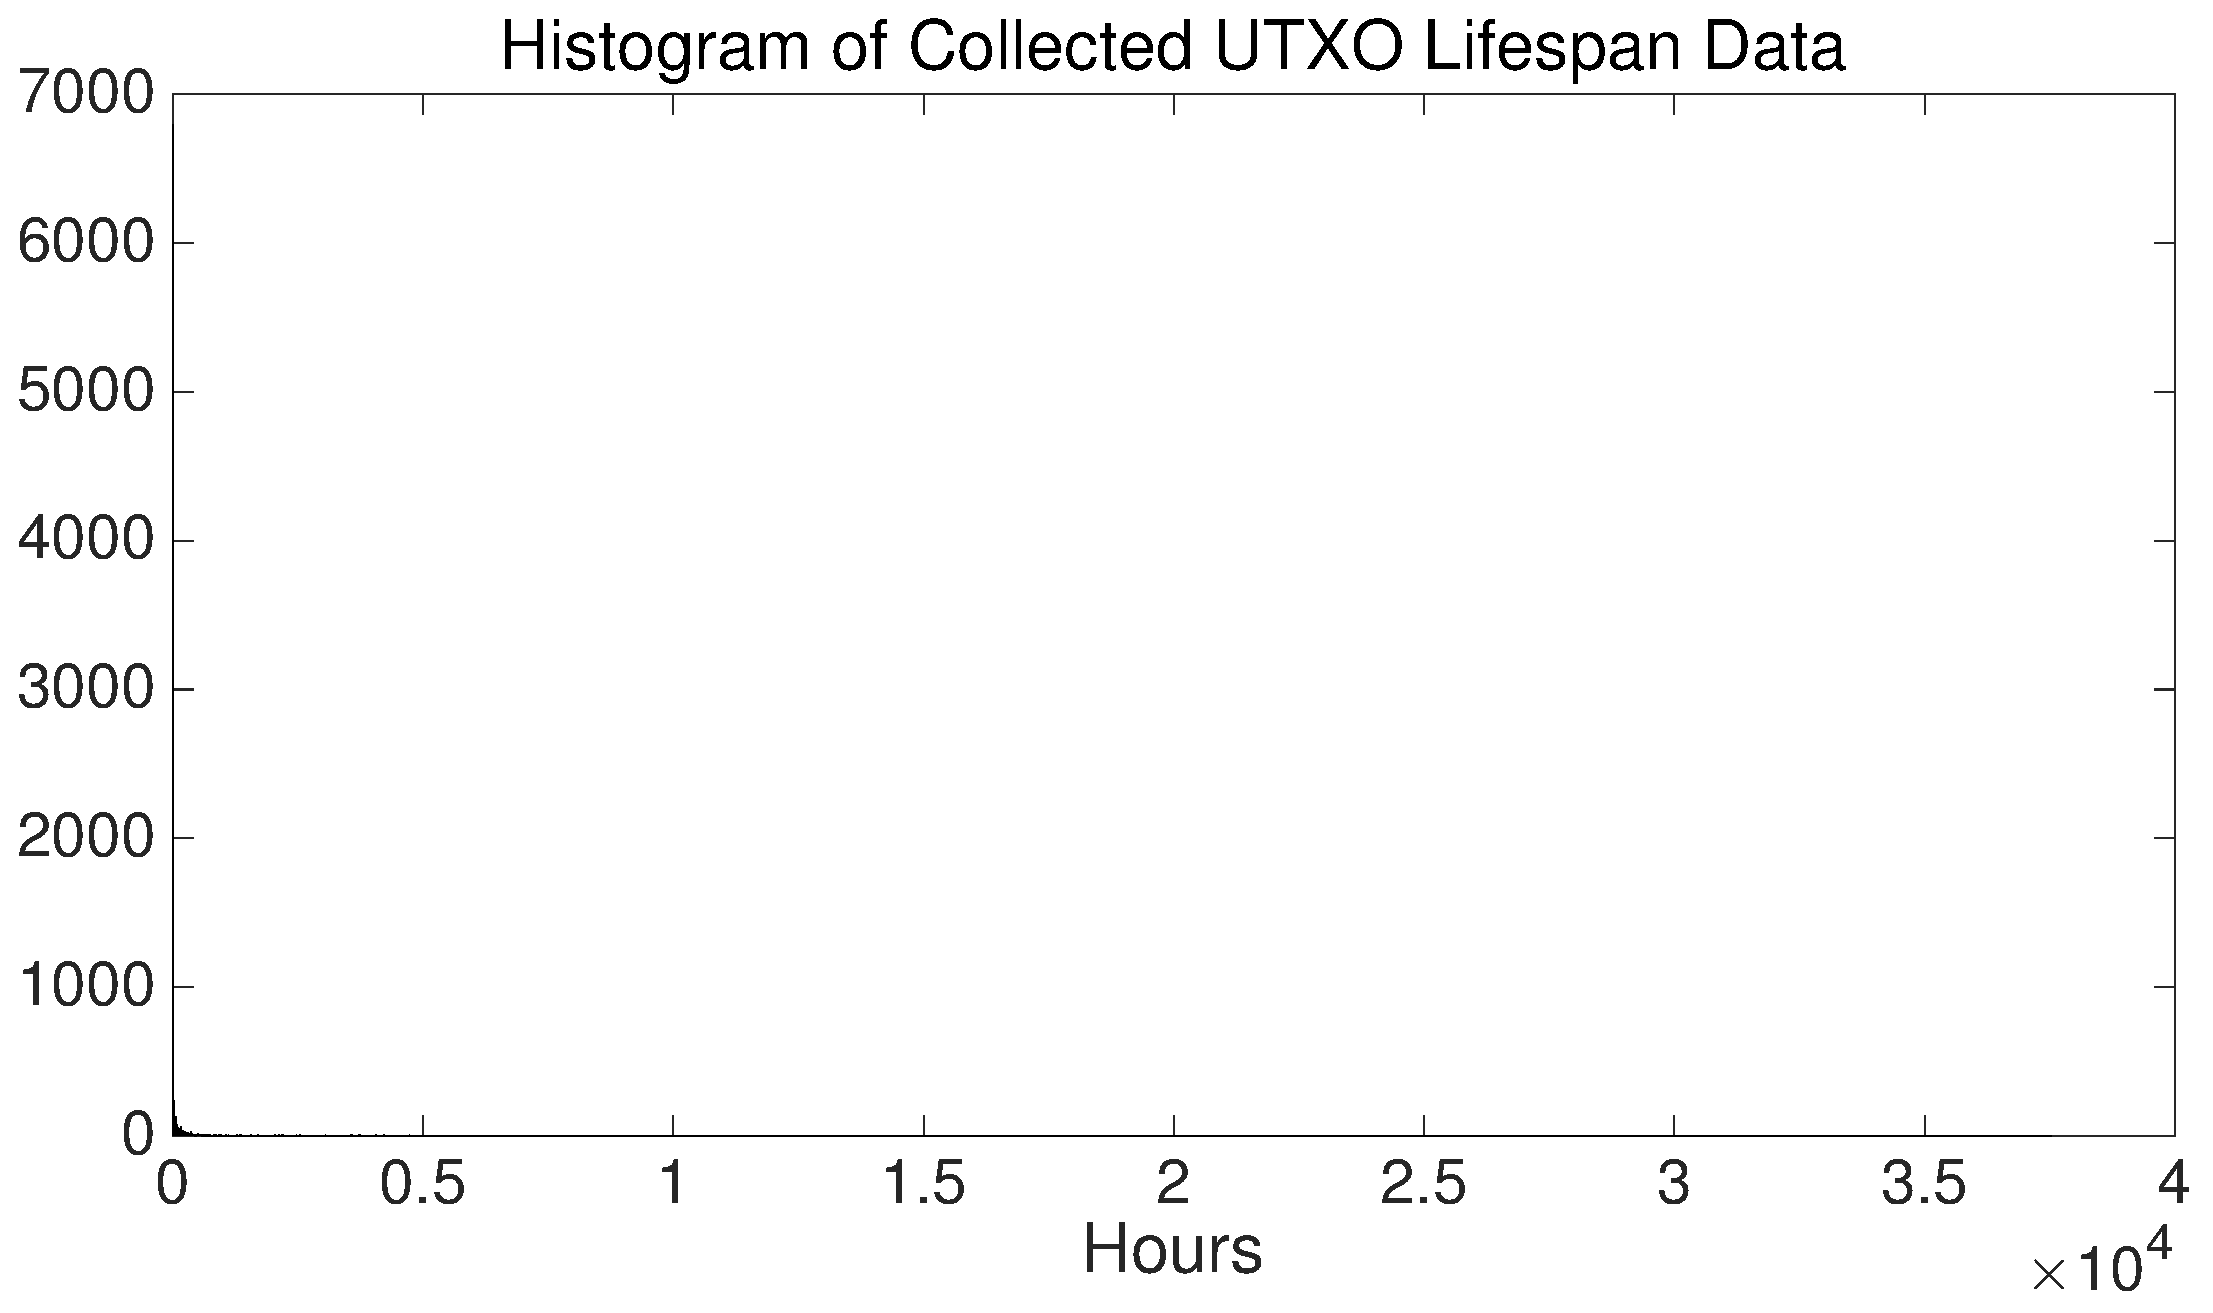
\includegraphics[width=0.8\textwidth]{figures/hist}
\end{center}
\caption{Histogram of 100 output values.}
\label{histogram}
\end{figure}
Every node in the Bitcoin network has a full copy of the blockchain
which, as previously mentioned, has every transaction that has ever
occurred. On the Stanford corn servers, we are running our own daemon
(node) that has a full copy of the blockchain that we are able to query
for relevant information. Unfortunately, this daemon did not make it
easy to gain the most important of all information for our problem: the
time (in blocks) that a transaction has been on the block chain. Figure~\ref{histogram} shows a histogram of some of these time periods. The mean of 100 points was 375 and the median was 96. Clearly there are many outliers.

We found it more convenient to use one of the (many) blockchain
explorers that have a public API exposing more information than our
daemon. Specifically we used the Blockchain.info explorer. Through HTTP
queries in python we were able to gather thousands of training examples
and export the data to the Matlab through the .mat data format, ready
for our classification algorithms. At the moment, we are using only a handful of training features - namely value, type of transaction (standard or non-standard), and locktime. 

\section*{Future Work}
We've written data collection scripts using bash and python but still need to run them to collect a few thousand data points. One of our collecting processes involves querying an API via HTTP and we are currently being throttled for over-querying. We plan on putting in a delay between each query and running the script over night.

We need to include more training features. A few more additions would be a better use of locktime, time of transaction (in UNIX time), number of inputs, number of peer outputs, and position in blockchain. These are all easy to find.

Since we have so few features, we would like to work with higher dimensioned implicit feature sets - \ie SVM Kernels. This is still not implemented.

\section*{Current Questions}
\begin{enumerate}
\item We would like to find more motivation for this idea. More specifically, who else would benefit from this predictor?
\item Since we're measuring time in integer block values, would it be better to use classification or regression?
\item Which Kernel is best for this?
\end{enumerate}



\newpage
\bibliography{template}

\end{document}